\chapter{线性单元和梯度下降}\label{chap:Line}

\begin{introduction}
	\item 线性单元是啥~\ref{Line:1}
	\item 线性单元的模型~\ref{Line:2}
	\item 监督学习和无监督学习~\ref{Line:3}
	\item 线性单元的目标函数~\ref{Line:4}
	\item 梯度下降优化算法~\ref{Line:5}
	\item $\nabla{E}({w})$的推导~\ref{Line:6}
	\item 随机梯度下降算法~\ref{Line:7}
	\item 编程实战:实现线性单元~\ref{Line:8}
\end{introduction}


在上一篇文章中,我们已经学会了编写一个简单的感知器,并用它来实现一个线性分类器。你应该还记得用来训练感知器的『感知器规则』。然而,我们并没有关心这个规则是怎么得到的。本文通过介绍另外一种『感知器』,也就是『线性单元』,来说明关于机器学习一些基本的概念,比如模型、目标函数、优化算法等等。这些概念对于所有的机器学习算法来说都是通用的,掌握了这些概念,就掌握了机器学习的基本套路。

\section{线性单元是啥}\label{Line:1}
感知器有一个问题,当面对的数据集不是\textbf{线性可分}的时候,『感知器规则』可能无法收敛,这意味着我们永远也无法完成一个感知器的训练。为了解决这个问题,我们使用一个\textbf{可导}的\textbf{线性函数}来替代感知器的\textbf{阶跃函数},这种感知器就叫做\textbf{线性单元}。线性单元在面对线性不可分的数据集时,会收敛到一个最佳的近似上。

为了简单起见,我们可以设置线性单元的激活函数$f$为$f(x)=x$, 这样的线性单元如图\ref{fig:Line1}所示,对比此前我们讲过的感知器如图\ref{fig:Line2}所示

\begin{figure}[h]
	\centering
	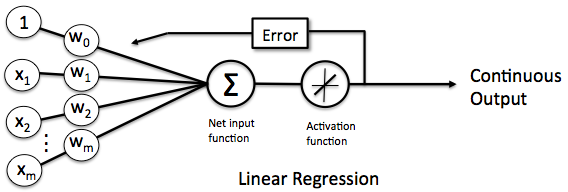
\includegraphics[width=0.7\textwidth]{Line1.png}
	\caption{线性单元}
	\label{fig:Line1}
\end{figure}

\begin{figure}[h]
	\centering
	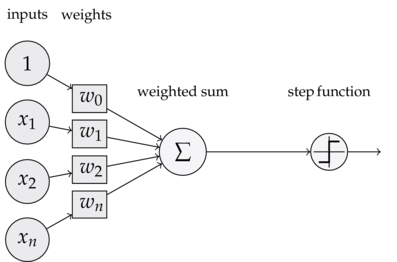
\includegraphics[width=0.5\textwidth]{Line2.png}
	\caption{感知器}
	\label{fig:Line2}
\end{figure}

这样替换了激活函数$f$之后,\textbf{线性单元}将返回一个\textbf{实数值}而不是\textbf{0, 1分类}。因此线性单元用来解决\textbf{回归}问题而不是\textbf{分类}问题。

\subsection{线性单元的模型}\label{Line:2}

当我们说\textbf{模型}时,我们实际上在谈论根据输入$x$预测输出$y$的\textbf{算法}。比如,$x$可以是一个人的工作年限,$y$可以是他的月薪,我们可以用某种算法来根据一个人的工作年限来预测他的收入。比如:
\[y=h(x)=w*x+b\]

函数$h(x)$叫做\textbf{假设},而$w$、$b$是它的\textbf{参数}。我们假设参数$w=1000$,参数$b=500$,如果一个人的工作年限是5年的话,我们的模型会预测他的月薪为
\[y=h(x)=1000*5+500=5500(\mbox{元})\]

你也许会说,这个模型太不靠谱了。是这样的,因为我们考虑的因素太少了,仅仅包含了工作年限。如果考虑更多的因素,比如所处的行业、公司、职级等等,可能预测就会靠谱的多。我们把工作年限、行业、公司、职级这些信息,称之为\textbf{特征}。对于一个工作了5年,在IT行业,百度工作,职级T6这样的人,我们可以用这样的一个特征向量来表示他
\[
	x = (\emph{5, IT, 百度, T6})
\]


既然输入$x$变成了一个具备四个特征的向量,相对应的,仅仅一个参数$w$就不够用了,我们应该使用4个参数\(w_1,w_2,w_3,w_4\),每个特征对应一个。这样,我们的模型就变成
\[y=h(x)=w_1*x_1+w_2*x_2+w_3*x_3+w_4*x_4+b\]

其中,\(x_1\)对应工作年限,\(x_2\)对应行业,\(x_3\)对应公司,\(x_4\)对应职级。

为了书写和计算方便,我们可以令\(w_0\)等于\(b\),同时令\(w_0\)对应于特征\(x_0\)。由于\(x_0\)其实并不存在,我们可以令它的值永远为1。也就是说
\[
	b = w_0 * x_0\qquad \mbox{其中} x_0=1
\]

这样上面的式子就可以写成
\begin{align*}
	y=h(x) & =w_1*x_1+w_2*x_2+w_3*x_3+w_4*x_4+b       \\
	       & =w_0*x_0+w_1*x_1+w_2*x_2+w_3*x_3+w_4*x_4
\end{align*}


我们还可以把上式写成向量的形式
\begin{equation}
	\label{eq:Line1}
	y=h(x)=w^Tx
\end{equation}



长成这种样子模型就叫做\textbf{线性模型},因为输出\(y\)就是输入特征\(x_1,x_2,x_3,...\)的\textbf{线性组合}。



\subsection{监督学习和无监督学习}\label{Line:3}

接下来,我们需要关心的是这个模型如何训练,也就是参数\(w\)取什么值最合适。

机器学习有一类学习方法叫做\textbf{监督学习},它是说为了训练一个模型,我们要提供这样一堆训练样本:每个训练样本既包括输入特征\(x\),也包括对应的输出\(y\)(\(y\)也叫做\textbf{标记,label})。也就是说,我们要找到很多人,我们既知道他们的特征(工作年限,行业...),也知道他们的收入。我们用这样的样本去训练模型,让模型既看到我们提出的每个问题(输入特征\(x\)),也看到对应问题的答案(标记\(y\))。当模型看到足够多的样本之后,它就能总结出其中的一些规律。然后,就可以预测那些它没看过的输入所对应的答案了。

另外一类学习方法叫做\textbf{无监督学习},这种方法的训练样本中只有\(x\)而没有\(y\)。模型可以总结出特征\(x\)的一些规律,但是无法知道其对应的答案\(y\)。

很多时候,既有\(x\)又有\(y\)的训练样本是很少的,大部分样本都只有\(x\)。比如在语音到文本(STT)的识别任务中,\(x\)是语音,\(y\)是这段语音对应的文本。我们很容易获取大量的语音录音,然而把语音一段一段切分好并\textbf{标注}上对应文字则是非常费力气的事情。这种情况下,为了弥补带标注样本的不足,我们可以用\textbf{无监督学习方法}先做一些\textbf{聚类},让模型总结出哪些音节是相似的,然后再用少量的带标注的训练样本,告诉模型其中一些音节对应的文字。这样模型就可以把相似的音节都对应到相应文字上,完成模型的训练。

\subsection{线性单元的目标函数}\label{Line:4}

现在,让我们只考虑\textbf{监督学习}。

在监督学习下,对于一个样本,我们知道它的特征\(x\),以及标记\(y\)。同时,我们还可以根据模型\(h(x)\)计算得到输出\(\bar{y}\)。注意这里面我们用\(y\)表示训练样本里面的\textbf{标记},也就是\textbf{实际值};用带上划线的\(\bar{y}\)表示模型计算的出来的\textbf{预测值}。我们当然希望模型计算出来的\(\bar{y}\)和\(y\)越接近越好。

数学上有很多方法来表示的\(\bar{y}\)和\(y\)的接近程度,比如我们可以用\(\bar{y}\)和\(y\)的差的平方的\(\frac{1}{2}\)来表示它们的接近程度
\[
	e=\frac{1}{2}(y-\bar{y})^2
\]

我们把\(e\)叫做\textbf{单个样本}的\textbf{误差}。至于为什么前面要乘\(\frac{1}{2}\),是为了后面计算方便。

训练数据中会有很多样本,比如\(N\)个,我们可以用训练数据中\textbf{所有样本}的误差的\textbf{和},来表示模型的误差\(E\),也就是
\[
	E=e^{(1)}+e^{(2)}+e^{(3)}+...+e^{(n)}
\]

上式的\(e^{(1)}\)表示第一个样本的误差,\(e^{(2)}\)表示第二个样本的误差......。

我们还可以把上面的式子写成和式的形式。使用和式,不光书写起来简单,逼格也跟着暴涨,一举两得。所以一定要写成下面这样

\begin{equation}
	\label{eq:Line2}
	E = e^{(1)}+e^{(2)}+e^{(3)}+...+e^{(n)}=\sum_{i=1}^{n}e^{(i)} =\frac{1}{2}\sum_{i=1}^{n}(y^{(i)}-\bar{y}^{(i)})^2
\end{equation}


其中
\begin{align*}
	\bar{y}^{(i)} =h(x^{(i)}) = w^T{x^{(i)}}
\end{align*}

公式\ref{eq:Line2}中,\(x^{(i)}\)表示第\(i\)个训练样本的\textbf{特征},\(y^{(i)}\)表示第\(i\)个样本的\textbf{标记},我们也可以用\textbf{元组}\((x^{(i)},y^{(i)})\)表示第\(i\)\textbf{训练样本}。\(\bar{y}^{(i)}\)则是模型对第\(i\)个样本的\textbf{预测值}。


我们当然希望对于一个训练数据集来说,误差最小越好,也就是公式\ref{eq:Line2}的值越小越好。对于特定的训练数据集来说,\((x^{(i)},y^{(i)})\)的值都是已知的,所以公式\ref{eq:Line2}其实是参数\({w}\)的函数。
\begin{align*}
	E({w}) =\frac{1}{2}\sum_{i=1}^{n}(y^{(i)}-\bar{y}^{(i)})^2 =\frac{1}{2}\sum_{i=1}^{n}({y^{(i)}-{w}^Tx^{(i)}})^2
\end{align*}


由此可见,模型的训练,实际上就是求取到合适的\({w}\),使(式2)取得最小值。这在数学上称作\textbf{优化问题},而\(E({w})\)就是我们优化的目标,称之为\textbf{目标函数}。


\subsection{梯度下降优化算法}\label{Line:5}

大学时我们学过怎样求函数的极值。函数\(y=f(x)\)的极值点,就是它的导数\(f'(x)=0\)的那个点。因此我们可以通过解方程\(f'(x)=0\),求得函数的极值点\((x_0,y_0)\)。

不过对于计算机来说,它可不会解方程。但是它可以凭借强大的计算能力,一步一步的去把函数的极值点『试』出来。如图\ref{fig:Line3}所示:


\begin{figure}[htbp]
	\centering
	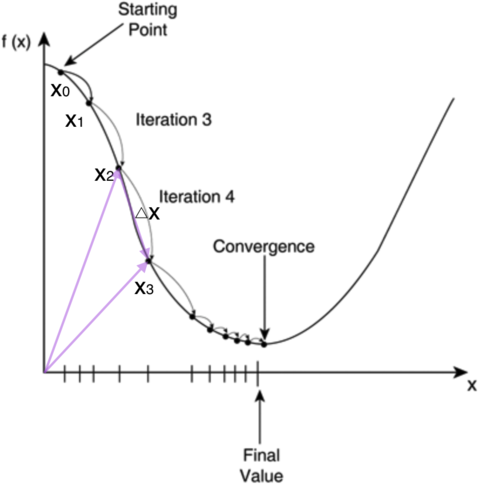
\includegraphics[width=0.6\textwidth]{Line3.png}
	\caption{极值点搜索图}
	\label{fig:Line3}
\end{figure}

首先,我们随便选择一个点开始,比如上图的\(x_0\)点。接下来,每次迭代修改\(x\)的为\(x_1,x_2,x_3,...\),经过数次迭代后最终达到函数最小值点。

你可能要问了,为啥每次修改\(x\)的值,都能往函数最小值那个方向前进呢?这里的奥秘在于,我们每次都是向函数\(y=f(x)\)的\textbf{梯度}的\textbf{相反方向}来修改\(x\)。什么是\textbf{梯度}呢?翻开大学高数课的课本,我们会发现\textbf{梯度}是一个向量,它指向\textbf{函数值上升最快}的方向。显然,梯度的反方向当然就是函数值下降最快的方向了。我们每次沿着梯度相反方向去修改\(x\)的
值,当然就能走到函数的最小值附近。之所以是最小值附近而不是最小值那个点,是因为我们每次移动的步长不会那么恰到好处,有可能最后一次迭代走远了越过了
最小值那个点。步长的选择是门手艺,如果选择小了,那么就会迭代很多轮才能走到最小值附近;如果选择大了,那可能就会越过最小值很远,收敛不到一个好的点
上。

按照上面的讨论,我们就可以写出梯度下降算法的公式
\[
	{x}_{new}={x}_{old}-\eta\nabla{f(x)}
\]
其中,\(\nabla\)是\textbf{梯度算子},\(\nabla{f(x)}\)就是指{}\(f(x)\)的梯度。\(\eta\)是步长,也称作\textbf{学习速率}。

对于上一节列出的目标函数(公式\ref{eq:Line2})
\[
	E({w})=\frac{1}{2}\sum_{i=1}^{n}({y^{(i)}-\bar{y}^{(i)}})^2
\]

梯度下降算法可以写成
\[
	{w}_{new}={w}_{old}-\eta\nabla{E({w})}
\]
聪明的你应该能想到,如果要求目标函数的\textbf{最大值},那么我们就应该用\textbf{梯度上升}算法,它的参数修改规则是
\[
	{w}_{new}={w}_{old}+\eta\nabla{E({w})}
\]

下面,请先做几次深呼吸,让你的大脑补充足够的新鲜的氧气,我们要来求取\(\nabla{E}({w})\),然后带入上式,就能得到线性单元的参数修改规则。

关于\(\nabla{E({w})}\)的推导过程,我单独把它们放到一节中。您既可以选择慢慢看,也可以选择无视。在这里,您只需要知道,经过一大串推导,目标函数\(E(w)\)的梯度是
\[
	\nabla{E({w})}=-\sum_{i=1}^{n}(y^{(i)}-\bar{y}^{(i)}){x}^{(i)}
\]

因此,线性单元的参数修改规则最后是这个样子
\begin{equation}
	{w}_{new}={w}_{old}+\eta\sum_{i=1}^{n}(y^{(i)}-\bar{y}^{(i)}){x}^{(i)}
	\label{eq:Line3}
\end{equation}


有了上面这个式子,我们就可以根据它来写出训练线性单元的代码了。

需要说明的是,如果每个样本有M个特征,则上式中的\({x},{w}\)都是M+1维\textbf{向量}(因为我们加上了一个恒为1的虚拟特征\(x_0\),参考前面的内容),而\(y\)是\textbf{标量}。用高逼格的数学符号表示,就是
\[
	{x},{w}\in\Re^{(M+1)},
	y\in\Re^1
\]

为了让您看明白说的是啥,我吐血写下下面这个解释(写这种公式可累可累了)。因为{}\({w},{x}\)是M+1维\textbf{列向量},所以(公式\ref{eq:Line3})可以写成
\begin{equation*}
	\begin{bmatrix}
		w_0 \\
		w_1 \\
		w_2 \\
		... \\
		w_m \\
	\end{bmatrix}_{new}=
	\begin{bmatrix}
		w_0 \\
		w_1 \\
		w_2 \\
		... \\
		w_m \\
	\end{bmatrix}_{old}+\eta\sum_{i=1}^{n}(y^{(i)}-\bar{y}^{(i)})
	\begin{bmatrix}
		1         \\
		x_1^{(i)} \\
		x_2^{(i)} \\
		...       \\
		x_m^{(i)} \\
	\end{bmatrix}
\end{equation*}
如果您还是没看明白,建议您也吐血再看一下大学时学过的《线性代数》吧。

\subsection{$\nabla{E}({w})$的推导}\label{Line:6}

这一节你尽可以跳过它,并不太会影响到全文的理解。当然如果你非要弄明白每个细节,那恭喜你骚年,机器学习的未来一定是属于你的。

首先,我们先做一个简单的前戏。我们知道函数的梯度的定义就是它相对于各个变量的\textbf{偏导数},所以我们写下下面的式子
\begin{align*}
	\nabla{E({w})} =\frac{\partial}{\partial{w}}E({w}) =\frac{\partial}{\partial{w}}\frac{1}{2}\sum_{i=1}^{n}(y^{(i)}-\bar{y}^{(i)})^2
\end{align*}
可接下来怎么办呢?我们知道和的导数等于导数的和,所以我们可以先把求和符号\(\sum\)里面的导数求出来,然后再把它们加在一起就行了,也就是
\begin{align*}
	\frac{\partial}{\partial{w}}\frac{1}{2}\sum_{i=1}^{n}(y^{(i)}-\bar{y}^{(i)})^2 = \frac{1}{2}\sum_{i=1}^{n}\frac{\partial}{\partial{w}}(y^{(i)}-\bar{y}^{(i)})^2
\end{align*}
现在我们可以不管高大上的\(\sum\)了,先专心把里面的导数求出来。
\begin{align*}
	\frac{\partial}{\partial{w}}(y^{(i)}-\bar{y}^{(i)})^2 = \frac{\partial}{\partial{w}}(y^{(i)2}-2\bar{y}^{(i)}y^{(i)}+\bar{y}^{(i)2})
\end{align*}
我们知道,\(y\)是与\({w}\)无关的常数,而\(\bar{y}={w}^T{x}\),下面我们根据链式求导法则来求导(上大学时好像叫复合函数求导法则)
\[
	\frac{\partial{E({w})}}{\partial{w}}=\frac{\partial{E(\bar{y})}}{\partial\bar{y}}\frac{\partial{\bar{y}}}{\partial{w}}
\]

我们分别计算上式等号右边的两个偏导数
\begin{align*}
	\frac{\partial{E({w})}}{\partial\bar{y}}=
	 & \frac{\partial}{\partial\bar{y}}(y^{(i)2}-2\bar{y}^{(i)}y^{(i)}+\bar{y}^{(i)2}) = -2y^{(i)}+2\bar{y}^{(i)} \\
	\frac{\partial{\bar{y}}}{\partial{w}}=
	 & \frac{\partial}{\partial{w}}{w}^T{x}= {x}
\end{align*}


代入,我们求得\(\sum\)里面的偏导数是
\begin{align*}
	\frac{\partial}{\partial{w}}(y^{(i)}-\bar{y}^{(i)})^2 = 2(-y^{(i)}+\bar{y}^{(i)}){x}
\end{align*}


最后代入\(\nabla{E}({w})\),求得
\begin{align*}
	\nabla{E({w})} =\frac{1}{2}\sum_{i=1}^{n}\frac{\partial}{\partial{w}}(y^{(i)}-\bar{y}^{(i)})^2 =\frac{1}{2}\sum_{i=1}^{n}2(-y^{(i)}+\bar{y}^{(i)}){x} =-\sum_{i=1}^{n}(y^{(i)}-\bar{y}^{(i)}){x}
\end{align*}


至此,大功告成。

\subsection{随机梯度下降算法}\label{Line:7}

如果我们根据(公式\ref{eq:Line3})来训练模型,那么我们每次更新\({w}\)的迭代,要遍历训练数据中所有的样本进行计算,我们称这种算法叫做\textbf{批梯度下降(Batch Gradient Descent)}。如果我们的样本非常大,比如数百万到数亿,那么计算量异常巨大。因此,实用的算法是SGD算法。在SGD算法中,每次更新\({w}\)的迭代,只计算一个样本。这样对于一个具有数百万样本的训练数据,完成一次遍历就会对\({w}\)更新数百万次,效率大大提升。由于样本的噪音和随机性,每次更新\({w}\)并不一定按照减少\(E\)的方向。然而,虽然存在一定随机性,大量的更新总体上沿着减少\(E\)的方向前进的,因此最后也能收敛到最小值附近。下图展示了SGD和BGD的区别

\begin{figure}[htbp]
	\centering
	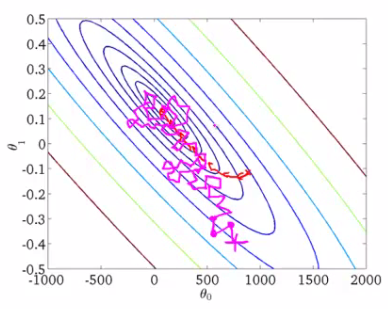
\includegraphics[width=0.7\textwidth]{Line4.png}
	\caption{极值点搜索图}
	\label{fig:Line4}
\end{figure}

如图\ref{fig:Line4},椭圆表示的是函数值的等高线,椭圆中心是函数的最小值点。红色是BGD的逼近曲线,而紫色是SGD的逼近曲线。我们可以看到BGD是一直向着最低点前进的,而SGD明显躁动了许多,但总体上仍然是向最低点逼近的。

最后需要说明的是,SGD不仅仅效率高,而且随机性有时候反而是好事。今天的目标函数是一个『凸函数』,沿着梯度反方向就能找到全局唯一的最小值。然而对于非凸函数来说,存在许多局部最小值。随机性有助于我们逃离某些很糟糕的局部最小值,从而获得一个更好的模型。


\section{编程实战:实现线性单元}\label{Line:8}

\begin{note}
	完整代码请参考GitHub: \url{https://github.com/hanbt/learn_dl/blob/master/linear_unit.py}
	(python2.7)
\end{note}

接下来,让我们撸一把代码。

因为我们已经写了感知器的代码,因此我们先比较一下感知器模型和线性单元模型,看看哪些代码能够复用。

\begin{table}[htbp]
	\centering
	\setlength{\tabcolsep}{7mm}
	\caption{模型函数对比}
	\begin{tabular}{ccc}
		\hline
		算法                                   & 感知器                             & 线性单元                           \\ \hline
		\multirow{2}{*}{\centering 模型$h(x)$} & $y=f(w^Tx)$                        & $y=f(w^Tx)$                        \\
		                                       & f(x) = 1*(z>0)                     & $f(z)=z$                           \\
		训练规则                               & \({w}\gets{w}+\eta(y-\bar{y}){x}\) & \({w}\gets{w}+\eta(y-\bar{y}){x}\) \\ \hline
	\end{tabular}
\end{table}

比较的结果令人震惊,原来除了激活函数\(f\)不同之外,两者的模型和训练规则是一样的(在上表中,线性单元的优化算法是SGD算法)。那么,我们只需要把感知器的激活函数进行替换即可。感知器的代码请参考第\ref{chap:Per}章,这里就不再重复了。对于一个养成良好习惯的程序员来说,重复代码是不可忍受的。大家应该把代码保存在一个代码库中(比如git)。
\begin{lstlisting}
from perceptron import Perceptron
#定义激活函数f
f = lambda x: x
class LinearUnit(Perceptron):
    def __init__(self, input_num):
        '''初始化线性单元,设置输入参数的个数'''
    Perceptron.__init__(self, input_num, f)
\end{lstlisting}

通过继承Perceptron,我们仅用几行代码就实现了线性单元。这再次证明了面向对象编程范式的强大。

接下来,我们用简单的数据进行一下测试。
\begin{lstlisting}
def get_training_dataset():
    '''
    捏造5个人的收入数据
    '''
    # 构建训练数据
    # 输入向量列表,每一项是工作年限
    input_vecs = [[5], [3], [8], [1.4], [10.1]]
    # 期望的输出列表,月薪,注意要与输入一一对应
    labels = [5500, 2300, 7600, 1800, 11400]
    return input_vecs, labels    
def train_linear_unit():
    '''
    使用数据训练线性单元
    '''
    # 创建感知器,输入参数的特征数为1(工作年限)
    lu = LinearUnit(1)
    # 训练,迭代10轮, 学习速率为0.01
    input_vecs, labels = get_training_dataset()
    lu.train(input_vecs, labels, 10, 0.01)
    #返回训练好的线性单元
    return lu
if __name__ == '__main__': 
    '''训练线性单元'''
    linear_unit = train_linear_unit()
    # 打印训练获得的权重
    print linear_unit
    # 测试
    print 'Work 3.4 years, monthly salary = %.2f' % linear_unit.predict([3.4])
    print 'Work 15 years, monthly salary = %.2f' % linear_unit.predict([15])
    print 'Work 1.5 years, monthly salary = %.2f' % linear_unit.predict([1.5])
    print 'Work 6.3 years, monthly salary = %.2f' % linear_unit.predict([6.3])
\end{lstlisting}

程序运行结果如下图:

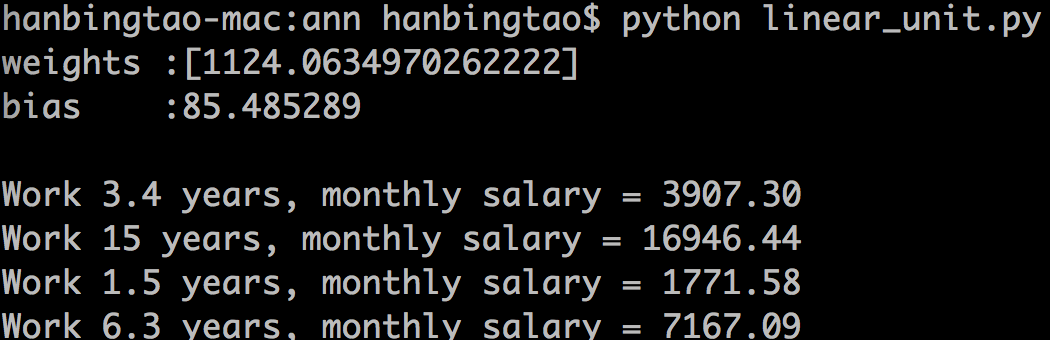
\includegraphics[width=0.7\textwidth]{Line5.png}


拟合的直线如下图:

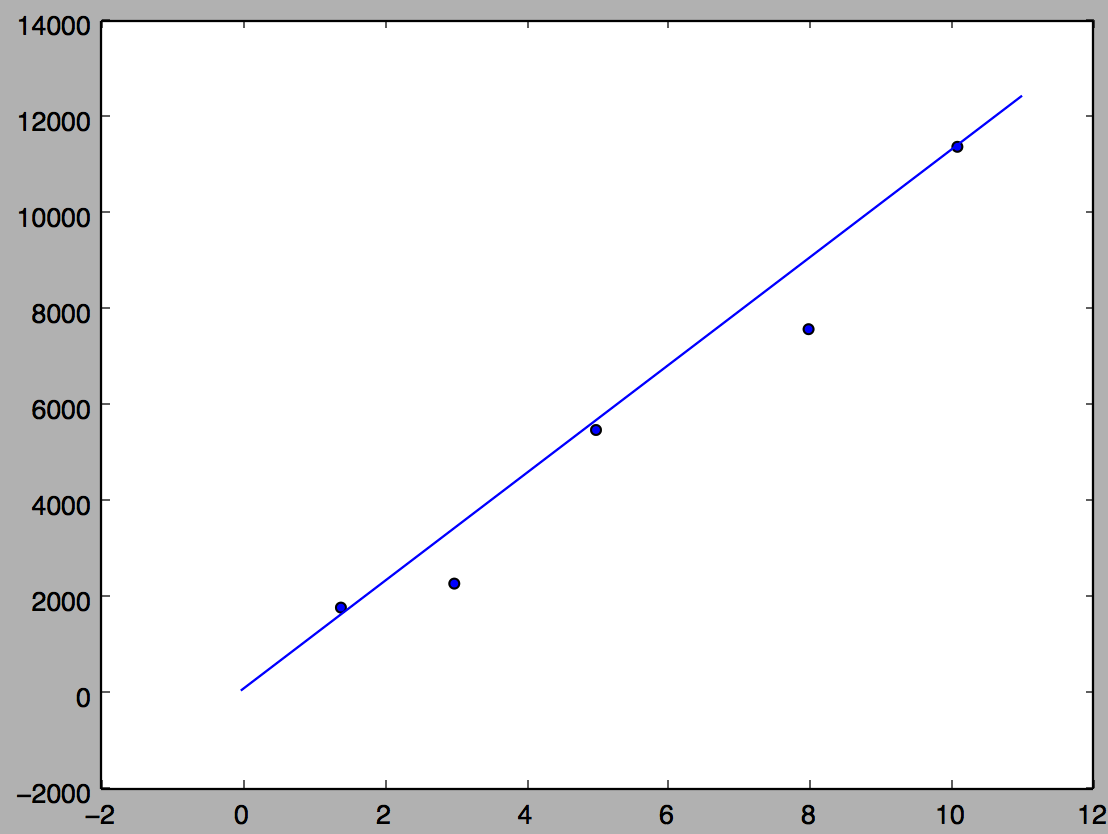
\includegraphics[width=0.7\textwidth]{Line6.png}


\section{小结}

事实上,一个机器学习算法其实只有两部分

\begin{itemize}
	\item
	      \emph{模型} 从输入特征\({x}\)预测输入\(y\)的那个函数\(h(x)\)
	\item
	      \emph{目标函数} 目标函数取最小(最大)值时所对应的参数值,就是模型的参数的\textbf{最优值}。很多时候我们只能获得目标函数的\textbf{局部最小(最大)值},因此也只能得到模型参数的\textbf{局部最优值}。
\end{itemize}

因此,如果你想最简洁的介绍一个算法,列出这两个函数就行了。

接下来,你会用\textbf{优化算法}去求取目标函数的最小(最大)值。\textbf{{[}随机{]}梯度\{下降\textbar 上升\}}算法就是一个\textbf{优化算法}。针对同一个\textbf{目标函数},不同的\textbf{优化算法}会推导出不同的\textbf{训练规则}。我们后面还会讲其它的优化算法。

其实在机器学习中,算法往往并不是关键,真正的关键之处在于选取特征。选取特征需要我们人类对问题的深刻理解,经验、以及思考。而\textbf{神经网络}算法的一个优势,就在于它能够自动学习到应该提取什么特征,从而使算法不再那么依赖人类,而这也是神经网络之所以吸引人的一个方面。

现在,经过漫长的烧脑,你已经具备了学习\textbf{神经网络}的必备知识。下一篇文章,我们将介绍本系列文章的主角:\textbf{神经网络},以及用来训练神经网络的大名鼎鼎的算法:\textbf{反向传播}算法。至于现在,我们应该暂时忘记一切,尽情奖励自己一下吧。



